\section{Security Implications}
\label{sec:sgx:security}

This section discusses the threat model,
how \graphenesgx{} defends against attacks from the untrusted OS,
and how users configure policies for defenses.
%for \sysn
% of the \graphenesgx{} framework, including the trusted and untrusted components,
%and the security implications of known \sgx{}-related threats to this framework.

%\subsection{Single-process, Linux COTS applications}

\subsection{Threat model}
\label{sec:sgx:overview:threat}

\graphenesgx{} follows a typical threat model for SGX applications.
The following components are untrusted:
(1) hardware outside of the Intel CPU package(s),
(2) the OS, hypervisor, and other system software,
(3) other applications executing on the same host, including unrelated enclaves,
and (4) user-space components that
reside in the application process but outside the enclave.
%Any of these untrusted components must be assumed malicious,
%and will constantly attempt to exploit
%any vulnerabilities on the interface of the trusted and untrusted components, to compromise the trusted components in any way possible.
Our design only trusts the CPUs and any code running inside the enclave, including the library OS, the unmodified application, and its supporting libraries. 
%\edit{Some code outside of the enclave is required, but not trusted.} %, and is needed for liveness but not for safety.}
%\graphenesgx{} places supporting code outside of the enclave, that is needed
%for liveness, but not safety.

%\fixmedp{pls check}
We also trust {\tt aesmd}, an enclave provided by the Intel's SGX SDK, which verifies
attributes in the enclave signature and approves the enclave creation.
%\fixmedp{please check the next sentence}
Currently, any framework that uses SGX for remote attestation must trust {\tt aesmd}.
\graphenesgx{} uses, but does not trust, the Intel SGX kernel driver.
%\edit{Any framework that uses SGX for remote attestation must also trust {\tt aesmd} for generating a cryptographic proof of the integrity of the Intel CPU.}
Other than {\tt aesmd} and the driver, \graphenesgx{} does not use or trust any part of the SDK.

%Any application that does remote attestation, including on \graphenesgx{}, must also trust {\tt AESMD},
%an enclave provided by Intel which implements remote attestation.

Denial of service, side channels, and controlled-channel attacks~\cite{xu15controlledchannel}
are vulnerabilities common to all SGX frameworks, and 
are beyond the scope of this work.
%\edit{Denial-of-service attacks by blocking CPU, memory, or IO resources are also beyond our scope.}



\subsection{User policy configuration}
\label{sec:sgx:overview:config}


Before an application is first executed using \graphenesgx{}, 
the user must make certain policy decisions.  
Our goal is to balance policy expressiveness
with usability.

As with Graphene and several other systems, each application requires a {\em manifest}
to specify which resources the application is allowed to use, including
a unioned, chroot-style view of the file system (comparable to aufs),
and a set of iptables-style network rules.
In Graphene, a program cannot access any resources not declared in the manifest.
The original intention of the manifest was to protect the host: a reference monitor 
can easily identify the resources an application might use, and reject an application
with a problematic manifest.

In \graphenesgx{}, the manifest is extended to protect the application from the host file system.
Specifically, the manifest can specify secure hashes (using SHA-256) of trusted files (generally read-only, including dynamic libraries). As part of opening a file,
\graphenesgx{} verifies the integrity of trusted files by checking the secure hashes.  A trusted file is only opened if the secure hash matches.
The manifest can also specify files or directories that can be accessed 
but are not trusted, such as a write-only output file.
\graphenesgx{} includes a signing utility that hashes all trusted files and 
generates a signed manifest that can be used at runtime.

SGX requires that certain resources be specified at initialization time, including the number of threads,
the maximum size of the enclave, and the starting virtual address of the enclave.  Thus, we also extend the manifest syntax for the 
user to specify these options.
Other security-sensitive manifest options inherited from \graphene{}, such as enabling debug output, are also protected as part of the signed manifest.



%%% Beyond the legacy threat model, we address new threats and challenges
%%% as the trade-offs for improving the \sgx{} usability and supporting Linux COTS applications in enclaves.
%%% For each application transited to \sgx{} by \graphenesgx{},
%%% a correspondent manifest file and enclave signature is provided by a trusted entity
%%% which has verified the application to be benign and authenticated the critical resources needed during its execution.
%%% The manifest file and enclave signature can be shipped and stored on an untrusted media, since the enclave signature also uniquely reflects manifest file.

\begin{comment}
\subsection{Provisioning and Attestation}

\fixmedp{We need a 1 para introduction to provisioning.  What is a provisioning server, and why do I need it?}

Once the \graphenesgx{} framework takes an application with its manifest file and enclave signature,
it creates an SGX enclave and step-by-step establishes
the trust of the remote provisioning server(s). 
We divide the process of trust establishment into three stages:

%When an application is loaded by \graphenesgx{}, it ought to be trusted by
%certain remote entities
%for provisioning confidential information or
%accepting the enclave's computation results.
%The trusted application code in the enclave includes both
%{\bf static} and {\bf dynamic} parts.
%The host ABI, library OS, and basic GNU lib C are loaded statically
%at the enclave launching time,
%with their integrity verified by the processor.
%Otherwise, any code that is dynamically loaded, or generated at runtime
%(e.g., by just-in-time compilation),
%must be secured by \graphenesgx{} or other trusted parts.


\begin{compactenum}

\item {\bf Isolated but not attested:}
Once \graphenesgx{} initializes the \libos{} and application binaries,
the application is successfully isolated within the enclave.
Ever since this stage, all components inside an enclave is mutually trusted:
The OS Shield is trusted to filter malicious input; the \libos{} and application binaries are trusted to maintain benign control flow and data access, and never bypass or corrupt the shield.


\item {\bf Isolated, attested, but not authenticated:}
When an enclave launched by \graphenesgx{} connects with a provisioning server,
\graphenesgx{} presents an attestation for the integrity
of the enclave---proving that the in-enclave execution is exactly derived from the application it claims to be. 
After this stage, the enclave is trusted by the provisioning server
that it runs the claimed application and not a malware.

\item {\bf Isolated, attested, and authenticated:}
At the last stage, the provisioning server can apply additional measures
to authenticate the locations, owners or credentials
of the attested enclave---an authenticated enclave is given absolute trust
to request and process any sensitive data with permission.


\end{compactenum}


Besides the components in the \graphenesgx{} framework,
an architectural enclave, {\tt AESMD}, introduced by the \sgxsdk{},
has to be trusted in our threat model.
The purpose of this enclave is to verify the attributes in enclave signatures
and generate a run-time token for initializing the enclave execution.
The {\tt AESMD} enclave is secured by a private key owned by Intel and the correspondent public key is recognized by all Intel CPUs with SGX.

%Besides the enclaves where applications are loaded,
%an architectural enclave called {\tt aesm} on each platform that supports SGX
%must be trusted by all enclave.
%{\tt AESM} is a secured service signed by Intel for generating
%valid enclave tokens.
%The {\tt aesm} binary is part of the \sgxsdk{},
%and signed using an Intel internal key, thus cannot be
%tampered by any third party.
%Otherwise, any other parts of the platform that launches the enclave
%must not be trusted, including the host kernel,
%\sgx{} kernel driver, and most parts of the hardware except the processor.



%\subsection{Remote Attestation and Secure Provisioning}
%
%For enclaves, the only way to be securely provisioned by another entity
%is by attestation.
%SGX provides a signed proof of the enclave measurement,
%which can be verified by other entities as long as their platforms
%also support SGX.
%In \haven{} model, the same shielding module cannot have different applications
%securely provisioned, because their enclave measurements will simply
%appear no difference.
%Because \graphenesgx{} includes the applications into enclave measurements,
%\sgx{} can generate attestation that differentiates the loaded applications,
%without any other guarantees from the shielding system.
\end{comment}



\subsection{Multi-process applications}
\label{sec:sgx:overview:multiproc}


\begin{figure}[t!]
\centering
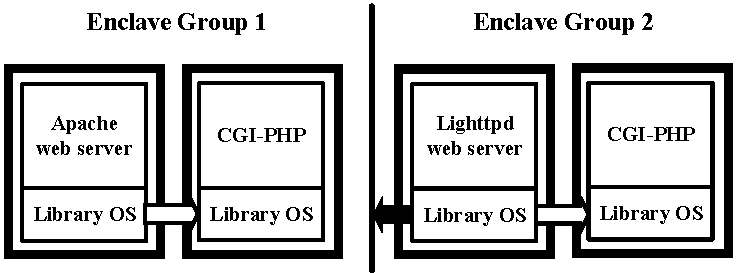
\includegraphics[width=.66\linewidth]{multiproc.pdf}
\caption{Two enclave groups, one running Apache and the other running Lighttpd, each creates a child enclave running CGI-PHP.
\graphenesgx{} distinguishes the child enclaves in different enclave groups.}
%As the child enclaves may appear the same for having the identical enclave signatures, the parent enclaves must distinguish their real children
%and defend against the untrusted host attempting to swap, duplicate or relay the child enclaves.}}
% The green (light) arrows represents the benign flow of inter-enclave communication, and the red (dark) arrow represent the flow that is manipulated by the untrusted host, or initiated by a malicious enclave group.}
\label{fig:multiproc-threats}
\end{figure}

Graphene supports multi-process applications by running
a separate library OS instance in each process~\cite{tsai14graphene}.
Each library OS instance coordinates state via message passing.
Graphene implements Linux multi-process abstractions in the user-space, including \syscall{fork}, \syscall{execve}, signals, and System V semaphores and message queues.

\graphenesgx{} extends the multi-process support of Graphene to enclaves by running each
process with a library OS instance in an enclave.
For instance, \syscall{fork} creates a second enclave
and copies the parent enclave's contents over message passing.
%except the child  library OS is adjusted with a different process ID.
%state adjusted slightly to
%give the child a different process ID. 
% migrated through message passing.
We call a group of coordinating enclaves an \emph{enclave group}.
Figure~\ref{fig:multiproc-threats} shows two mutually-untrusting enclave groups running on a host.


Because multi-process abstractions are implemented in enclaves,
securing these abstractions from the OS is straightforward. 
\graphenesgx{} adds: %The primary pieces we add for multi-processing support are:
(1) the ability for enclaves to authenticate each other via local attestation,
and thereby establish a secure channel,
and (2) a mechanism to securely fork into a new enclave, adding the child to the enclave group (see Section \ref{sec:sgx:shield:multiproc}).


%% \graphenesgx{} spans a multi-process application across multiple enclaves.
%% Despite other alternatives of fitting multiple executables into single enclave,
%% \graphenesgx{} uses an ``one-enclave-per-process'' strategy to isolate multi-process applications.
%% This design decision is based on two reasons: (1) The majority of Linux COTS applications contain position-dependent executables, which have to be loaded at a specific address (often at {\tt 0x400000}). (2) Most applications partitioned as multiple executables assume separation of address spaces across processes.


%\graphenesgx{} puts the enclaves created by the same application instance into an {\bf enclave group}.
%Within an enclave group, all the enclaves are mutually trusting each other,
%to share OS states across \libos{} instances.
%On the other hand, enclaves that
%belongs to different enclave groups are mutually untrusting units,
%and \graphenesgx{} strictly blocks sharing
%any state across enclave groups.


%% We anticipate new challenges in retaining the security isolation when extending single-enclave execution into multi-enclave. Figure~\ref{fig:multiproc-threats} shows a classic example with the problems. First of all, the OS shield within each enclave now has to shield inter-enclave communication, which is more complex than shielding resources for single enclave. A malicious can make the attack attempt on an enclave group,
%% by pretending, swapping or relaying one of the enclaves, whereas the enclaves cannot coordinate through sharing enclave memory.
%% The enclaves in an enclave group must establish trusted paths
%% for authenticating each other, to prevent being compromised by the untrusted host. 


%For multi-process applications, each process created by \graphenesgx{}
%will be isolated in its own enclave.
%By default, no trust is required between the processes,
%unless the {\bf manifest} specifies any policy
%that allows sharing multi-process abstractions.
%For example, a parent process can decide to pass output to a child process
%through a secured pipe,
%but the parent process does not have to trust the child, assuming
%the parent will sanitize any information passed to the child.
%For processes that have the same security level,
%clients can also put them into a mutually trusted group, where all processes are allowed to share any abstractions.


%\fixmedp{This subsection isn't adding much (a lot of philosophy that isnt' directly relevant; cutting for now}

\begin{comment}
\subsection{Verification and authentication}


Despite that most applications hosted by
an App store, package repository or software channel are designed to be benign 
and not for the attacking purpose,
it is impractical to assume any applications taken off-the-shelf
to be bug-free and invulnerable to exploitation.
All of the legacy frameworks including the \sdk{} and shielding systems
require trusting the isolated applications,
that they will never expose vulnerabilities that will lead to leaking the sensitive data or corrupting the in-enclave execution.
Their threat models mostly assume
developers' involvement in verifying the invulnerability of applications and authenticating the run-time resources.


\graphenesgx{} retains the model of
verifying an application ahead-of-time before signing it off for enclave isolation.
Despite that relying on manual verification by the developers
is still an option, we argue that it is feasible to automate the verification process.





\subsection{Side-channel Attacks}

Preventing the enclaves from leaking side-channel information to the untrusted hosts is extremely challenging.
%Since enclaves are launched on untrusted hosts, it is hard to prevent
%enclaves from becoming vulnerable to side-channel attacks.
Attackers may exploit timing channels or implicit information flow to expose the protected data in the enclave, and current \sgx{} technology has no effective strategy to defend against them.

A recent work~\cite{xu15controlledchannel} shows that a even stronger
side-channel attack to applications running
inside enclaves exists, which is referred as the {\bf controlled channel attack}.
A controlled channel attack is
an amplified side-channel attack---it exploits the fact that an enclave relies on the untrusted operating system for page management.
A malicious OS can manipulate paging to trigger page faults on every instructions in the enclave,
and exploit the partial information of the top 54 bits of the faulting addresses, to expose more secrets.
%the OS can manipulate paging to reinforce the side channels
%for exposing more secrets.
%So far there is no  against this type of attacks, except minimizing
%the side channels by rearranging code and data in enclave pages.

Both side-channel attacks and controlled channel attacks are problems common to \sgx{} frameworks.
We assumes solving these attacks out of the scope.

\end{comment}
